\chapter{CONCEITOS E TÉCNICAS NECESSÁRIAS}

Neste capítulo é feita uma revisão de assuntos relacionados, visando embasamento conceitual, para o entendimento deste trabalho.

\section{Testes manuais}

Hoje, com o notável crescimento da demanda e a constante mudança do mercado, e consequentemente as necessidades das empresas, surge a importância dos softwares acompanharem estas mudanças tanto na rapidez, quanto na qualidade. Mas como se garante a qualidade de um software? Um dos caminhos são os testes \cite{PRESSMAN}. Com eles pode-se obter a certeza, do que foi desenvolvido ou modificado, não resultará em nenhuma falha tanto na fase de desenvolvimento quanto na de produção.

Existem dois tipos de testes: o automático e o manual, no qual neste tópico, são explanados os testes manuais. Os testes manuais são aqueles em que pessoas são alocadas especialmente para testar o sistema, na busca por erros, como por exemplo, clicar em todos os links para testar suas respectivas integridades, escrever caracteres especiais em campos que não deveriam aceitá-lo para ver se o sistema realmente detectará esta falha, etc. Imagine um sistema que acesse um banco de dados, por exemplo. O teste deve cobrir a chamada pela interface de usuário, passando pelas camadas de negócio até chegar no banco. Este método, comparado com os testes automatizados, é um processo mais falho por este ser mais lento, de desempenho inferior e por consumir muito mais tempo. Para \citeonline{PRESSMAN}, alguns programas, mesmo que pequenos, podem apresentar problemas ao serem testados, por estes possuírem uma grande quantidade de possibilidades a ser executada. Como exemplificado por \citeonline{PRESSMAN}, ``[...] um programa PASCAL de 100 linhas com um único laço que pode ser executado não mais do que 20 vezes. Há aproximandamente $10^{14}$ caminhos que podem ser executados!'' Com isso, o número de pessoas para realizar testes manuais e ter um retorno satisfatório seria grande, o que consequentemente, aumentaria o custo do projeto.

Outro problema é quando novas funcionalidades são adicionadas ao programa, o que obriga a execução de todos os testes novamente, fazendo com que todo procedimento seja repetido, acarretando um grande desperdício de tempo.

\section{Desenvolvimento Orientado a Testes}

Desenvolvimento Orientado a Testes ou \textit{Test-Driven Development} (TDD), é uma abordagem para desenvolvimento de software que consiste na criação do teste antes do código (\textit{test-first}) e refatoração do mesmo. Sua filosofia pode ser resumida em uma frase: somente escreva código para fazer um teste falho passar \cite{KOSKELA}. O fluxograma do ciclo do TDD é apresentado na Figura \ref{tdd}:

\begin{figure}[ht]
    \centering
    \scalebox{0.7}{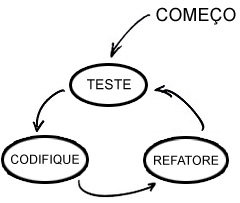
\includegraphics{figuras/tdd}}
    \caption{Fluxograma do ciclo do TDD}
    \label{tdd}
\end{figure}

\citeonline{ASTELS} define o TDD como um estilo de desenvolvimento onde:
\begin{itemize}
    \item{É mantida uma suíte exaustiva de testes;}
    \item{Nenhum código entra em produção a menos que possua testes associados que o valide;}
    \item{Os testes são escritos primeiro;}
    \item{Os testes determinam que código é preciso escrever.}
\end{itemize}

TDD causa grande impacto na qualidade de um software. \citeonline{BECK} nos auxilia no entendimento dessa premissa ao afirmar que:
\begin{itemize}
    \item{Toda vez que alguém toma uma decisão e não a testa, existe uma grande probabilidade de que esta decisão esteja errada;}
    \item{Funcionalidades de software que não podem ser demonstradas através de testes automatizados simplesmente não existem;}
    \item{Testes nos dão à chance de pensar sobre o que é desejado, independente da forma como a solução será implementada.}
\end{itemize}

De forma geral, ao utilizarmos TDD, deve-se escrever um sólido conjunto de testes, denominado suíte de testes, para a verificação do correto funcionamento do sistema. Esta suíte deverá, idealmente, cobrir todo o código do sistema, provendo confiabilidade ao processo de desenvolvimento de software. Vale ressaltar, que TDD não garante a obtenção de níveis aceitáveis em certos aspectos do software final, como usabilidade, desempenho, entre outros. Muito disto, se deve ao fato de TDD não conseguir extinguir riscos relacionados com a falta, ou definição equivocada, de requisitos \cite{RIBEIRO}.

\section{Sistemas de controle de versão}

Uma das ações mais importantes para permitir que diversos desenvolvedores trabalhem juntos em um mesmo projeto é utilizar um Sistema de Controle de Versão (SCV), também conhecido como ``repositório de código'' ou simplesmente ``repositório''. Existem muitos desses sistemas disponíveis no mercado, tais como Subversion, Rational ClearCase, Mercurial, Git, entre outros.

Devido as suas vantagens, os SCVs são sistemas utilizados em muitos tipos de projetos, desde os de pequeno porte aos de grande porte, mostrando a importância desses sistemas. Por isso, atualmente, é difícil encontrar um projeto profissional que não use um Sistema de Controle de Versão, ainda mais com a quantidade de softwares livres que constam nessa área e a imensa qualidade que eles apresentam.

Os Sistemas de Controle de Versão fornecem um local para armazenamento dos arquivos de um projeto e também controlam as versões dos mesmos, possibilitando que desenvolvedores trabalhem no mesmo arquivo ao mesmo tempo \cite{SHORE}. Imagine, por exemplo, que em um projeto haja uma classe Calculadora com capacidade apenas de listar e calcular o valor da soma entre dois números, e que o programador implemente multiplicação e divisão entre dois números. Ao armazenar o código atualizado com as novas funcionalidades, o repositório grava uma nova versão desta classe, ou seja, a classe Calculadora original não é simplesmente substituída por uma nova, ao invés disso, o novo código é anexado ao antigo.

No SCV também é possível guardar versões dos arquivos, possibilitando a recuperação dos mesmos de forma análoga a um botão de ``desfazer''. Quando ocorre algum tipo de erro em um arquivo e este é colocado acidentalmente no repositório, este mecanismo nos permite desfazer as alterações do último \textit{commit} (envio das modificações feitas pelo usuário ao repositório de código), e obter o arquivo antigo \cite{SHORE}. Voltando ao exemplo da classe Calculadora, imagine que a primeira versão funcionasse perfeitamente e, ao ser implementada a multiplicação e divisão entre dois números, algum tipo de erro fosse introduzido por falta de atenção. Suponha ainda que este erro só fosse percebido quando a classe já estivesse em produção. Nesse tipo de situação, a possibilidade de controlar versões com um SCV é muito útil, porque permite a obtenção de uma versão anterior rapidamente (a que funcionava) e colocá-la em produção até que a versão mais recente (com problemas) seja corrigida.

\section{Métodos ágeis}

Cansados de fazer software da mesma maneira, um grupo de desenvolvedores se reuniu para discutir sobre formas de aumentar o desempenho de seus projetos. Desta reunião, alguns valores e princípios foram definidos e, com base neles, foi criado o Manifesto Ágil, que pode ser visto na Figura \ref{manifesto_agil}. ``O Manifesto Ágil, criado em 2001, descreve a essência de um conjunto de abordagens para desenvolvimento de software criadas ao longo da última década'' \cite{IMPROVEIT-MANIFESTO}. Dos valores e princípios do Manifesto Ágil são baseados os métodos ágeis de desenvolvimento de software, que contrastam com a maneira tradicional de se desenvolver.

\begin{figure}[ht]
    \centering
    \scalebox{0.7}{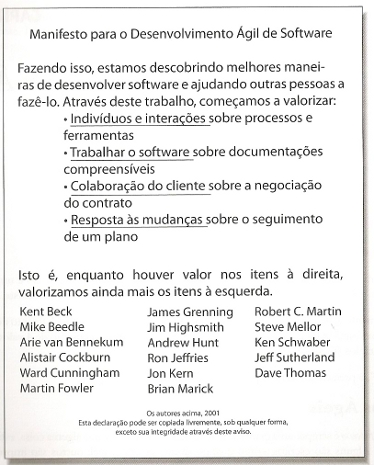
\includegraphics{figuras/manifesto_agil}}
    \caption{Manifesto Ágil. Fonte: \cite{SHORE}}
    \label{manifesto_agil}
\end{figure}

Dos métodos ágeis mais populares, como Scrum, Lean, Crystal, entre outros, uma das metodologias de desenvolvimento que mais se popularizou foi a \textit{Extreme Programming} (XP). Esta, criada por Kent Beck em 1999, é amplamente utilizada em inúmeros projetos ao redor do mundo.

O XP é composto por valores e práticas, e uma destas práticas é a Integração Contínua, tema abordado neste trabalho. A Integração Contínua é uma técnica que foi amplamente difundida com os métodos ágeis \cite{DUVALL-ENTREVISTA}, o que não quer dizer que esta surgiu e somente se encaixa com os métodos ágeis. \citeonline{DUVALL-ENTREVISTA} relata que já trabalhou em projetos que usavam o ciclo de vida ``Cascata'' e, mesmo assim, a equipe utilizava Integração Contínua.

Outros métodos ágeis não possuem como prática a Integração Contínua, porém, são facilmente adaptáveis. O Scrum, por exemplo, não tem a Integração Contínua como prática nativa, mas é perfeitamente adaptável.

